\section{はじまり}
梅雨も明け空気に茹るような暑気と夏の香を帯びた時候。午後を迎えた聖MIDI女学園中等部、一般の生徒は昼食を終えたあとの微睡みと奮闘しながら授業を受けている。
そして、生徒会室では、ロージアがスマートフォンを片手に神妙な面持ちで深沈している。
\ \\
\kao{fig/rosia.png}{うむむ…}\\
\kao{fig/holmy.png}{ロージアどうしたんですか? 珍しく真面目な顔をして…}\\
\kao{fig/rosia.png}{珍しくって何よ、あざと学ダンス主席で成績もと~っても優秀なロージアちゃんはいつも真面目です~}\\
\kao{fig/tsukino.png}{ろーじあはテストでいい点とってるし、とっても真面目なの~}\\
\kao{fig/rosia.png}{やっぱりツキノはちゃんと私のこと見てくれてるね♪ いつもありがと$\heartsuit$ お兄ちゃんはロージアちゃんのこと見てくれる…?(謎カメラ目線)}\\
\kao{fig/holmy.png}{(誰にいってるんですか…)}\\
\kao{fig/jacklyn.png}{ロージアが真面目かはともかく、そんな顔でスマホみてるなんて珍しいやん? どうしたん?}\\
\kao{fig/rosia.png}{どうしたもこうしたも無いわよ、今度の台風見た?}\\
\kao{fig/holmy.png}{台風69号でしたっけ…}\\
\kao{fig/rosia.png}{そうそう、それね。その台風が今度のライブに来るかもしれないのよ}\\
\kao{fig/jacklyn.png}{ほんまか!? せっかくうちらも練習しとるし、見に来るファンのおにいやん達も現場のスタッフさんたちの為にも何事もなかったように開催してほしいなぁ…}\\
\kao{fig/tsukino.png}{台風ってすぐにあぶないってわかったりしないの?}\\
\kao{fig/rosia.png}{そうよね~最近はえーあい…? が流行ってるし、なんとかなりそうだけどね。ねえねえホルミー、そういうの作れたりしないの?}\\
\kaot{fig/holmy.png}{『そういうの』って…天気予報ですら当てることが難しいのによく言いますね…\\
でも、ライブだけでなく電車を早めに止めたりの意思決定にも使えそうですし、作ってみる価値はあるかもしれませんね。私たちは寮だから登校はあまり関係なさそうですけど…}\\
\kaot{fig/rosia.png}{なるほどね、AIが止めれば簡単に休校になるってことでしょ$\heartsuit$ 
面白そうじゃん、ホルミー、AIの作り方を教えて~$\heartsuit$}\\
\kao{fig/holmy.png}{えっ、私ですか…!? AIを作るための数学なら教えられますけど…}\\
\kao{fig/rosia.png}{えー数学ー…ま、全然大丈夫だけどね$\heartsuit$}\\
\kao{fig/tsukino.png}{つきの、すーがく苦手なの…}\\
\kao{fig/rosia.png}{つきのはあまり数学とかは得意そうじゃないよね、ロージアちゃんが教えてあげるわ$\heartsuit$}\\
\kao{fig/jacklyn.png}{ロージアが数学得意ってなんか珍しいやん}\\
\kao{fig/rosia.png}{まあね~これでもホルミー直々に鍛えてもらったからね~\footnotemark[1]}
\footnotetext[1]{以前の作品「ろーほるすーがくれっすん」のこと
\\ \url{https://irisu-in-wonderland.tumblr.com/post/156533872627}}\\
\kao{fig/jacklyn.png}{ええな~うちもホルミーに数学教えてもらいたいわぁ~}\\
\kao{fig/holmy.png}{ええっと…はじめたいのですが…}\\
\[
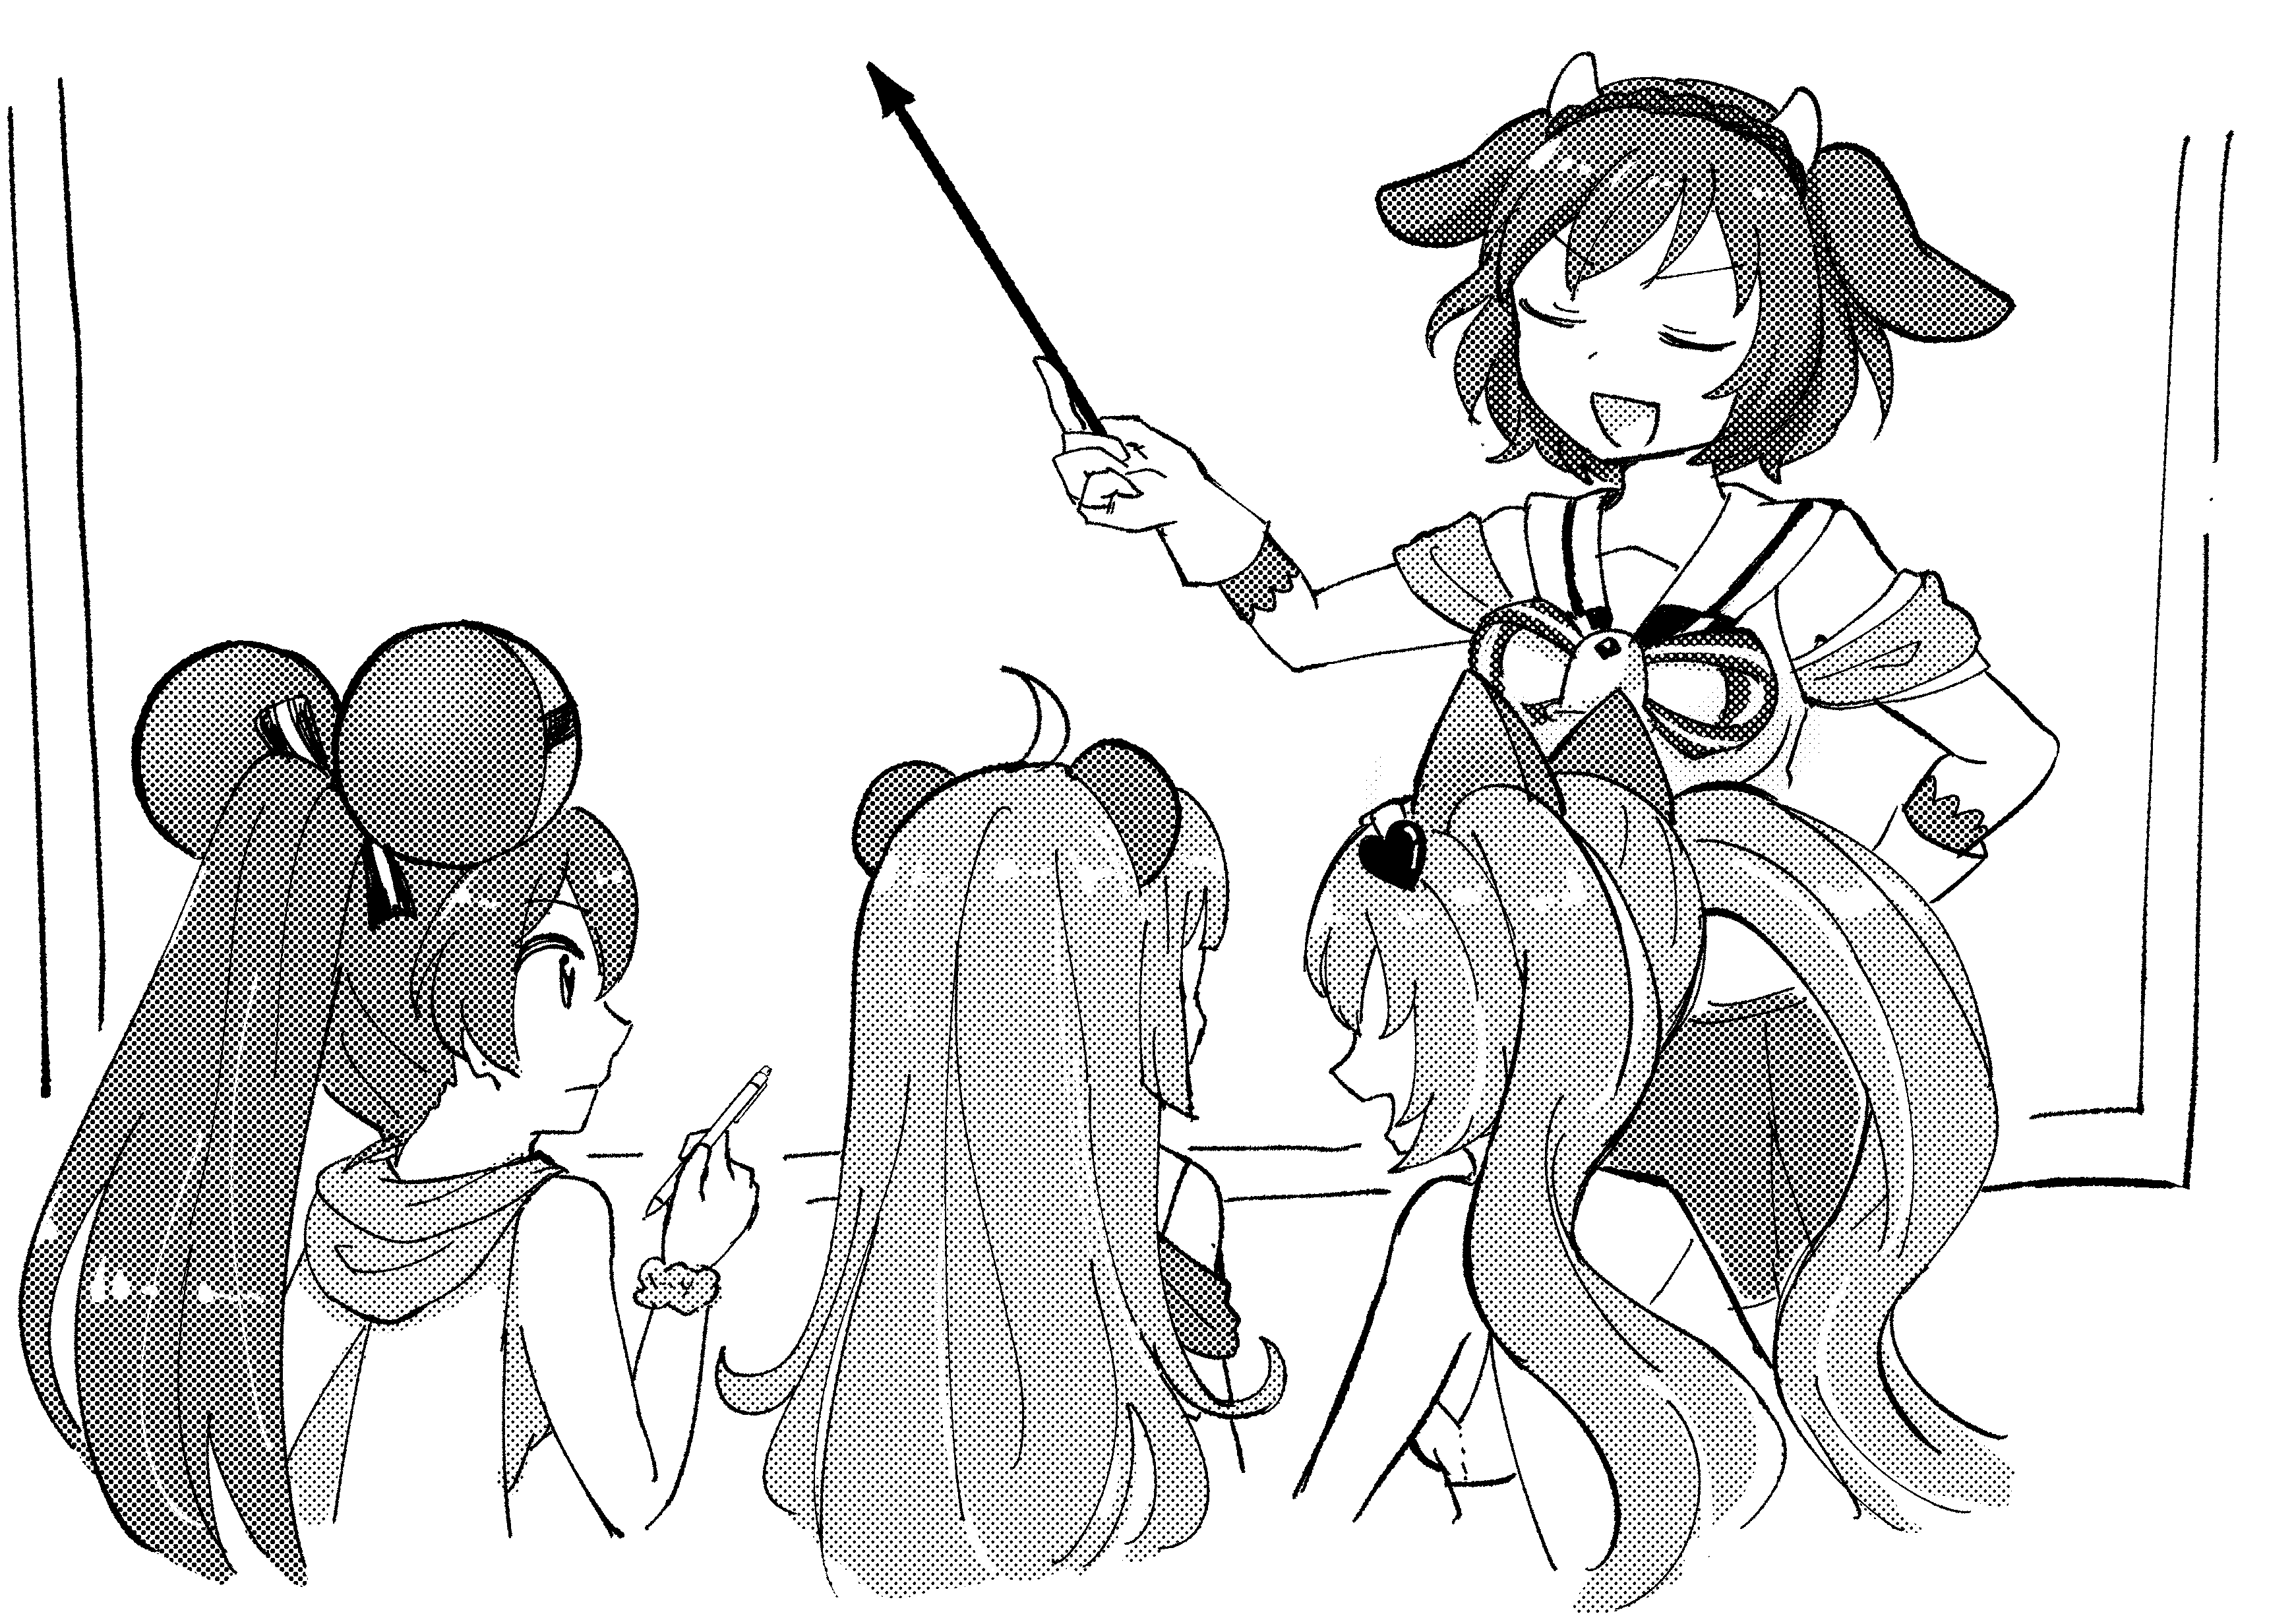
\includegraphics[width=1.\textwidth]{fig/lesson_start.png}
\]
